\chapter{Un'Introduzione ai Transformers}

\section{Contextualized Embeddings}

\dfn{Meaning Conflation Problem}{
Gli algoritmi di distribuzione basati sulla similarità racchiudono tutti i sensi di una parola in un unico embedding (anche quando sono diversi). 
}

\nt{Per risolvere questo problema sono state introdotte le reti di transformers/transformers network (TNs).}

\dfn{Contextualized Embeddings}{
  Le TNs hanno lo scopo di apprendere contextualized embeddings i cui significati cambiano in base al contesto in cui i termini appaiono. Ogni parola riceve un contextualized embedding che è la media pesata di qualche embeddings di input (simile a word2vec)
}

\paragraph{Le TNs consistono di uno stack a più strati:}

\begin{itemize}
  \item L'embeddings di output per lo strato $i$ diventa l'input embeddings dello strato $i + 1$. 
  \item Solitamente gli strati variano tra 2 e 24. 
  \item Più livelli performano meglio permettendo alla rete di apprendere funzioni più complesse.
\end{itemize}

\subsection{Architettura}

L'input entra nell'encoder del transformer attraverso uno strato di attention e uno trato di FeedForward Network (FFN). L'output entra nel decoder  attraverso due strati di attention e uno di FFN.

\begin{figure}[h]
    \centering
    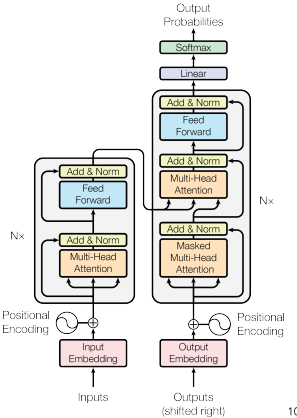
\includegraphics[scale=0.5]{06/transf.png}
    \caption{Architettura attuale di un transformer.}
\end{figure}

\paragraph{Transformer originale:}

\begin{itemize}
  \item Il modello originale era uno stack a 6 strati. 
  \item L'output dello strato $l$ è l'input dello strato $l + 1$ finché non è stata raggiunta la predizione finale.
\end{itemize}

\dfn{Encoder}{
  L'encoder è composto da uno stack di 6 strati identici ognuno di esso composto da due sottostrati:
  \begin{itemize}
    \item Un meccanismo multi-head di self-attention. 
    \item Una semplice FFN.
  \end{itemize}
  Attorno a ogni sottostrato sono applicati:
  \begin{itemize}
    \item Residual Connection: si somma l'input orginale del sottostrato con il suo output. 
    \item Normalizzazione.
  \end{itemize}
}

\nt{Per facilitare l'applicazione della residual connection ogni sottostrato e strato produce vettori con la stessa dimensione.}

\dfn{Decoder}{
  Il decoder è composto da uno stack di 6 strati identici, ognuno dei quali contiene tre sottostrati:
  \begin{itemize}
    \item Un meccanismo multi-head di self-attention con mascheramento per impedire l'accesso a posizioni future nella sequenza.
    \item Un meccanismo multi-head di attenzione sull'output dell'encoder.
    \item Una semplice FFN.
  \end{itemize}
  Attorno a ogni sottostrato sono applicati:
  \begin{itemize}
    \item Residual Connection: si somma l'input originale del sottostrato con il suo output.
    \item Normalizzazione.
  \end{itemize}
}

\nt{Il mascheramento nella self-attention del decoder assicura che la predizione alla posizione $i$ dipenda solo dalle posizioni precedenti, non da quelle future.}

\paragraph{Ogni strato implementa una sequenza di operazioni tra cui:}

\begin{itemize}
  \item Aggiungere informazione posizionale all'input degli embeddings: l'embedding di ogni parola cambia in base alla sua posizione nel testo in input.
  \item \fancyglitter{Self-attention:} Vengono generati embedding che sono la media pesata degli embedding nello stage precedente. 
  \item Somma e normalizzazione.
\end{itemize}

\paragraph{Tipi di Transformers:}

\begin{itemize}
  \item \fancyglitter{Encoder-only:} convertono una sequenza di testo in input in una rappresentazione numerica dove la rappresentazione calcolata per un dato token dipende sia dal contesto sinistro che da quello destro (bidirectional attention). BERT e derivati appartengono a questa categoria. 
  \item \fancyglitter{Decoder-only:} completano un dato input predicendo iteramente la parola più probabile (autoregressive attention). In questa categoria rientrano i modelli GPT. 
  \item \fancyglitter{Encoder-Decoder:} utilizzati per modellare mapping complessi, solitamente in traduzione e sommarizzazione. E.g. BART.
\end{itemize}

\subsection{Strati}

\dfn{Feed-Forward Sublayer}{
  Il sottostrato Feed-Forward (FFN) viene applicato dopo i meccanismi di attenzione e ha due obiettivi principali:
  \begin{itemize}
    \item Permette la trasformazione non lineare delle rappresentazioni, introducendo complessità nel modello.
    \item Aiuta ad apprendere caratteristiche astratte, come ruoli sintattici, classi semantiche o categorie latenti (es. tipi di verbi, entità nominate).
  \end{itemize}
  Viene applicato posizione per posizione in modo indipendente, ed è composto da due layer lineari separati da una funzione di attivazione non lineare (tipicamente ReLU).
}

\nt{Apprende attraverso backpropagation, ma solitamente non da etichette a livello di token.}

\paragraph{Questo strato:}

\begin{itemize}
  \item Si occupa di apprendere trasformazioni intermedie della rappresentazione dei token che sono utili per obiettivo finale. 
  \item Per esempio: 
    \begin{itemize}
      \item Ruoli sintattici: soggetto, oggetto, etc. 
      \item Ruoli semantici: agente, paziente, luogo, etc. 
      \item Enfatzzare caratteristiche salienti: polarità, tensione, etc. 
      \item Creare clusters.
    \end{itemize}
\end{itemize}

\dfn{Self-attention}{
  La self-attention è lo strumento che permette di associare chi sta parlando di cosa.
}

\nt{Esempio: "The animal didn't cross the street because it was too tired.", la self-attention ci dice che "it" si riferisce ad "animal".}

\dfn{Positional Encoding}{
  È un modo per tener conto dell'ordine delle parole in una sequenza di input. Il transformer aggiunge un vettore a ogni input embedding. Questi vettori seguono uno specifico pattern che il modello impara per determinare la posizione di ogni parola o la differenza tra parole diverse in una sequenza.
}

\dfn{Encoder-Decoder Attention}{
  Il meccanismo di attenzione encoder-decoder permette al decoder di focalizzarsi sulle parti rilevanti dell'input. In questo sottostrato:
  \begin{itemize}
    \item I vettori di Key ($K$) e Value ($V$) sono ottenuti dall’output dell’encoder.
    \item I vettori di Query ($Q$) sono ottenuti dal layer inferiore del decoder.
  \end{itemize}
  Funziona come un'attenzione multi-head standard, ma incrocia le rappresentazioni:
  \begin{itemize}
    \item le Query vengono dal decoder, mentre Keys e Values provengono dall’encoder.
  \end{itemize}
  Questo consente al decoder di accedere direttamente all’informazione contestuale dell’input durante la generazione dell’output.
}

\begin{figure}[h]
    \centering
    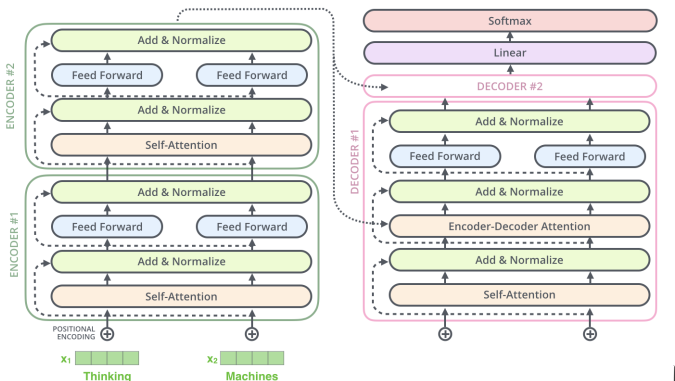
\includegraphics[scale=0.5]{06/ed.png}
    \caption{Encoder-Decoder.}
\end{figure}

\section{Training}

Quando si va a fare training su un dataset etichettato si può valutarne l'output confrontandlo con quello corretto. 

\dfn{Loss Function}{
  La loss function (funzione di perdita) misura quanto le predizioni del modello si allontanano dalla realtà (cioè, dalla sequenza corretta).
}

\begin{figure}[h]
    \centering
    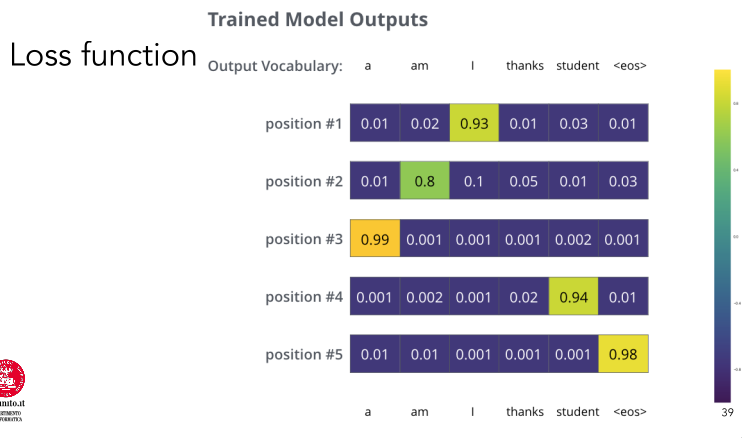
\includegraphics[scale=0.5]{06/loss.png}
    \caption{Loss Function.}
\end{figure}

\begin{figure}[h]
    \centering
    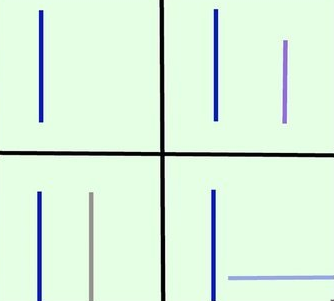
\includegraphics[scale=0.5]{06/loss2.png}
    \caption{"Loss" Function.}
\end{figure}

\subsection{Positional Embeddings}

\dfn{Positional Embeddings}{
  Nei Transformer, l’ordine delle parole non è implicito, perciò si aggiunge una rappresentazione della posizione di ciascuna parola.
  \begin{itemize}
    \item Ogni parola $w_i$ ha un embedding standard $w_i$ e una rappresentazione di posizione $p_i$.
    \item L’embedding finale in input è dato dalla somma: $x_i = w_i + p_i$.
  \end{itemize}
  A differenza di approcci precedenti che concatenavano la posizione come vettore separato, nei Transformer la posizione è integrata direttamente nel vettore parola.
  \begin{itemize}
    \item La funzione $p_i$ è definita in modo deterministico (hard-coded), tipicamente tramite funzioni sinusoidali che variano in modo unico per ogni posizione.
  \end{itemize}
}

\nt{Le positional embeddings forniscono al modello informazioni sul contesto sequenziale, pur mantenendo l'architettura completamente parallela del Transformer.}

\begin{figure}[h]
    \centering
    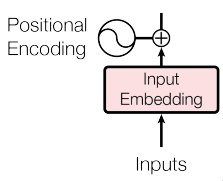
\includegraphics[scale=0.5]{06/emb.png}
    \caption{Positional Encoding.}
\end{figure}

\dfn{Positional Encoding}{
  I positional encodings sono definiti in modo deterministico tramite funzioni seno e coseno di frequenze diverse. Per una posizione $pos$ e una dimensione $i$:
  \[
  \text{PE}_{(pos, 2i)} = \sin\left(\frac{pos}{10000^{\frac{2i}{d_{\text{model}}}}}\right)
  \quad
  \text{PE}_{(pos, 2i+1)} = \cos\left(\frac{pos}{10000^{\frac{2i}{d_{\text{model}}}}}\right)
  \]
  \begin{itemize}
    \item Le dimensioni pari del vettore usano la funzione seno.
    \item Le dimensioni dispari usano la funzione coseno.
    \item $d_{\text{model}}$ è la dimensione del modello (es. 512).
  \end{itemize}
}
\nt{L’uso di funzioni sinusoidali permette al modello di apprendere relazioni tra posizioni tramite semplici operazioni lineari, e generalizzare a lunghezze di sequenza mai viste.}

\subsection{Sub-word Tokenization}

\dfn{Sub-word Tokenization}{
  I Transformer operano su unità sub-word, ovvero frammenti di parole piuttosto che parole intere. Queste unità sono generate automaticamente mediante l'algoritmo di Byte Pair Encoding (BPE):
  \begin{itemize}
    \item Il vocabolario iniziale contiene tutti i singoli caratteri, inclusi simboli speciali come \texttt{</w>} per indicare la fine di una parola.
    \item L’algoritmo scansiona un corpus di testo e conta le coppie di simboli più frequenti.
    \item La coppia più frequente viene sostituita con la sua concatenazione e aggiunta al vocabolario come nuovo simbolo.
    \item Questo processo viene ripetuto iterativamente, costruendo un dizionario di unità sub-word che cattura sequenze frequenti.
  \end{itemize}
}

\paragraph{La sub-word tokenization:}

\begin{itemize}
  \item Rendono la TN più \fancyglitter{robusta} quando incontra parole sconosciute: utilizzando delle sottoparole conosciute. 
  \item Salva spazio: si utilizza un vocabolario molto più piccolo.
\end{itemize}

\subsection{Attention}

\dfn{Multi-Head Attention}{
  Il meccanismo di multi-head attention permette al modello di focalizzarsi su diverse parti della sequenza in parallelo. Ogni testa $h_n$ utilizza tre proiezioni:
  \begin{itemize}
    \item Query ($Q$): vettore che rappresenta la parola corrente e cerca informazioni rilevanti nelle altre parole. Dimensione $d_q = 64$.
    \item Key ($K$): vettore associato a ogni parola, che consente di determinare quanto essa debba essere presa in considerazione. Dimensione $d_k = 64$.
    \item Value ($V$): vettore che contiene l'informazione effettiva che può essere “letta” se la parola è rilevante. Dimensione $d_v = 64$.
  \end{itemize}
  L’attenzione di ogni testa è calcolata come:
  \[
  \mathrm{Attention}(Q, K, V) = \mathrm{softmax}\left(\frac{QK^\top}{\sqrt{d_k}}\right)V
  \]
  Dopo il calcolo parallelo di 8 teste indipendenti, i risultati vengono concatenati e proiettati in uno spazio di dimensione $d_{\text{model}} = 512$.
}

\nt{La TNs espandono lo strato dell'attention ripetendolo più volte.}

\dfn{Self-Attention}{
  Il meccanismo di self-attention consente a ogni parola della sequenza di “osservare” tutte le altre parole e combinare le loro rappresentazioni in modo pesato.
  \begin{itemize}
    \item Per ogni parola $w_i$ si generano tre vettori: 
    \begin{itemize}
      \item Query ($q_i$)
      \item Key ($k_i$)
      \item Value ($v_i$)
    \end{itemize}
    \item I vettori $q_i$ e $k_j$ vengono usati per calcolare uno score di attenzione tra la parola $w_i$ e ogni altra parola $w_j$.
    \item Lo score determina quanto $w_i$ deve “prestare attenzione” a $w_j$.
    \item L’embedding finale $z_i$ di $w_i$ è una combinazione pesata dei vettori $v_j$ delle altre parole, in base ai punteggi di attenzione.
  \end{itemize}
}

\paragraph{L'intuizione può essere spiegata con un'analogia:}

\begin{itemize}
  \item La query è un tipo particolare di pane. 
  \item Le chiavi sono il nome di tutti i prodotti della panetteria. 
  \item Il valore di ogni prodotto è il prezzo.
\end{itemize}

\nt{L'obiettivo è di porre più attenzione al prezzo (values) dei prodotti (keys) che sono più vicini ai nostri interessi (query).}

\subsection{Training}

\dfn{Training}{
  L’addestramento di un Transformer consiste nell’ottimizzare i suoi parametri:
  \begin{itemize}
    \item gli embedding di input dei token sub-word,
    \item le matrici di pesi $W$ nei diversi layer (es. proiezioni di Q, K, V e FFN).
  \end{itemize}

}
\paragraph{Il processo di training si articola in due fasi:}

  \begin{itemize}
    \item \fancyglitter{Pre-training (non supervisionato)}: il modello apprende rappresentazioni linguistiche generali da grandi quantità di testo, tipicamente usando compiti come il masked language modeling.
    \item \fancyglitter{Fine-tuning (supervisionato)}: il modello viene specializzato per un compito specifico (es. classificazione, traduzione, Q\&A) utilizzando un dataset etichettato.
  \end{itemize}

\cor{Pre-training (MLM)}{
  Le procedure di pre-training permettono di catturare una serie di languages pattern che sono indipendenti dall'applicazione. I modelli di pre-training utilizzano un Masked Languag Model (MLM): 
  \begin{itemize}
    \item I tokens sono mascherati rimpiazzandoli con token speciali (e.g $[$MASK$]$) e la TN deve indovinare il token sotto la maschera. 
    \item Solitamente un 15\% dei tokens viene mascherato. 
  \end{itemize}
}

\begin{figure}[h]
    \centering
    
\includegraphics[scale=0.3]{06/mlm.png}
    \caption{MLM or something idk.}
\end{figure}

\paragraph{MLM:}

\begin{enumerate}
  \item Il classificatore che predice la masked word funziona al di sopra del contextualized embedding prodotto dallo strato $n$. 
  \item Il pre-training è un algoritmo non supervisionato perché non richiede annotazioni da esperti del dominio. 
  \item I masked tokens possono apparire dovunque in un dato testo. Un contesto che può essere usato per indovinarli sia da destra che da sinistra della maschera è chiamato \fancyglitter{bidirectional language model}\footnote{Tradizionalmente gli LM procedono da sinistra a destra.}.
\end{enumerate}

\cor{Pre-training (NSP)}{
Un'altra procedura per il pre-training è il next sentence prediction (NSP). I transformers sono allenati a predire quali frasi seguono da una frase data in input. 
}

\paragraph{NSP:}

\begin{itemize}
  \item Utilizzano Token e Positional embeddings. 
  \item Utilizzano un nuovo tipo di embedding che codifica a quale segmento il current token appartiene. 
  \item Viene introdotto il token $[$CLS$]$ che viene inserito all'inizio dell'input: 
     \begin{itemize}
    \item È trattato come un normale token: partecipa alla self-attention con tutti gli altri token.
    \item La sua rappresentazione contestualizzata (embedding finale) viene usata come input per un classificatore.
    \item Grazie all’attenzione,  accumula informazioni da tutta la sequenza.
  \end{itemize}
\item Genera esempi positivi dalla frase presa in esame ed esempi negativi da pezzi a caso del corpus. 
\end{itemize}

\dfn{Fine-Tuning}{
  Il fine-tuning consiste nell’adattare un Transformer pre-addestrato a un compito specifico di NLP:
  \begin{itemize}
  \item I testi di input sono preceduti da $[$CLS$]$ e separati, se necessario, da $[$SEP$]$.
    \item Il modello di base è già stato pre-addestrato (e.g. con MLM o NSP).
    \item Si prosegue l’addestramento con una funzione di loss specifica per il task, per esempio cross-entropy per la classificazione.
  \end{itemize}
}

\paragraph{Problemi:}

\begin{itemize}
  \item L'attention algorithm ha complessità quadratica. 
  \item Solitamente non è un problema perché si usa il parallelismo delle GPU, ma quando queste non sono disponibili le TNs sono molto più lenti di semplici reti neurali. 
  \item I positional embeddings codificano posizioni assolute dei token, anche se nuove architetture implementano un sistema relativo.
\end{itemize}
